\documentclass{beamer}
\usetheme{Boadilla}
\usepackage{tikz}
\usetikzlibrary{calc}


\title{Organic compound}
\subtitle{From Wikipedia}
\author{Stefan van Deventer}
\institute{University of Stellenbosch}
\date{\today}


\begin{document}
\begin{frame}
	\titlepage
\end{frame}

\begin{frame}
	\frametitle{Overview}
	\tableofcontents
\end{frame}


%-----------------------------------------------
\section{History}
\begin{frame}
	The name "organic" is a historical name from the 19th century.
	%\vspace
	\newline
	\newline
	People believed that only living things could make organic compounds and "dead" things (such as minerals) 
	could make inorganic compounds. However, Friedrich Wöhler proved this wrong by synthesizing urea, a well-known 
	organic compound.
\end{frame}
%\pause
\begin{frame}
	There are natural organic compounds, and synthetic ones. Their structure may be described by using names, 
	and making diagrams.
	%\space
	\begin{block}{Showing}
		One way of showing the molecule is by drawing its structural formula. Because molecules can have 
		complicated structures, people have made ways to show them in simple language. One way is to use line 
		diagrams. Each atom is shown by a letter, and connected by a line to each atom with which it is has a 
		covalent bond. One line means a single bond, two lines means a double bond and so on.
	\end{block}
	%\vspace
	Because there is in an infinite number of possible organic compounds, language is needed to give a 
	unique name to each one. The International Union of Pure and Applied Chemistry, or IUPAC, made a system for 
	doing this.

	\end{frame}

%-----------------------------------------------
\section{Natural Compounds}
\begin{frame}
	Although an IUPAC name makes every single possible molecule unique, the names are often long and complicated, 
	so in everyday life, trivial names--unofficial but widely understood names--are used, such as the trivial 
	names Paracetamol, Tylenol, and Acetaminophen, which are used for a compound whose IUPAC name is 
	N-(4-hydroxyphenyl) acetamide. Some of these trivial names are trademarks.

	\begin{figure}
	\begin{equation}
		\binom{x}{n} = \frac{x^2}{n!} = \frac{x(x-1) \cdots (x-n+2)(x-n+1)}{n(n-1) \cdots 2 \cdot1}
	\end{equation}
	\begin{equation}
		N_{t} = N_{0} + \int_{0}^{t} \Phi_{s} dM_{s}
	\end{equation}
	\end{figure}

\end{frame}
\begin{frame}
	\begin{itemize}
		\item Mass spectrometry
		\item X-ray diffraction
		\item Nuclear magnetic resonance spectroscopy
		\item Infrared spectroscopy
	\end{itemize}
\end{frame}


%-----------------------------------------------
\section{Diagram}
\begin{frame}
	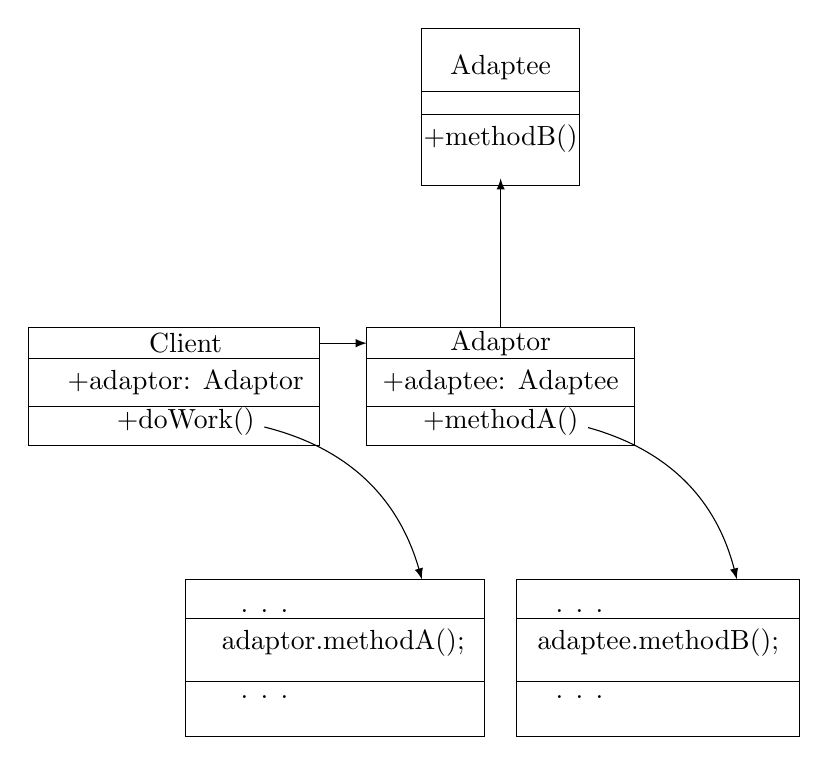
\begin{tikzpicture}[scale=1]

	\node[minimum size=1cm, node distance=3cm] (Adaptee) at (6,8.5) {Adaptee};
	\node[minimum size=1cm, node distance=3cm] (methodB) at (6,7.6) {+methodB()};
	\draw (5,7) -- (5,9) -- (7,9) -- (7, 7) -- cycle;
	\draw (5,8.2) -- (7, 8.2);
	\draw (5,7.9) -- (7, 7.9);

	\node[minimum size=1cm, node distance=3cm] (Adaptor) at (6,5) {Adaptor};
	\node[minimum size=1cm, node distance=3cm] (adap) at (6,4.5) {+adaptee: Adaptee};
	\node[minimum size=1cm, node distance=3cm] (methodA) at (6,4) {+methodA()};
	\draw (4.3,3.7) -- (4.3,5.2) -- (7.7,5.2) -- (7.7, 3.7) -- cycle;
	\draw (4.3,4.8) -- (7.7,4.8);
	\draw (4.3,4.2) -- (7.7,4.2);

	\node[minimum size=1cm, node distance=3cm] (Client) at (2,5) {Client};
	\node[minimum size=1cm, node distance=3cm] (adap2) at (2,4.5) {+adaptor: Adaptor};
	\node[minimum size=1cm, node distance=3cm] (doWork) at (2,4) {+doWork()};
	\draw (0,3.7) -- (0,5.2) -- (3.7,5.2) -- (3.7, 3.7) -- cycle;
	\draw (0,4.8) -- (3.7,4.8);
	\draw (0,4.2) -- (3.7,4.2);

	\draw[->,>=latex] (6,5.2) -- (methodB);
	\draw[->,>=latex] (3.7,5) -- (4.3,5);

	\draw[->,>=latex] (doWork) to[bend left] (5,2);
	\draw[->,>=latex] (methodA) to[bend left] (9,2);

	\node[minimum size=1cm, node distance=3cm] (AdapA) at (4,1.2) {adaptor.methodA();};
	\node[minimum size=1cm, node distance=3cm] (AdapB) at (8,1.2) {adaptee.methodB();};
	\draw (2,0) -- (2,2) -- (5.8,2) -- (5.8, 0) -- cycle;
	\draw (2,1.5) -- (5.8,1.5);
	\draw (2,0.7) -- (5.8,0.7);

	\draw (6.2,0) -- (6.2,2) -- (9.8,2) -- (9.8, 0) -- cycle;
	\draw (6.2,1.5) -- (9.8,1.5);
	\draw (6.2,0.7) -- (9.8,0.7);

	\node[minimum size=1cm, node distance=3cm] (dots1) at (3, 1.6) {. . .};
	\node[minimum size=1cm, node distance=3cm] (dots2) at (3, 0.5) {. . .};

	\node[minimum size=1cm, node distance=3cm] (dots3) at (7, 1.6) {. . .};
	\node[minimum size=1cm, node distance=3cm] (dots4) at (7, 0.5) {. . .};

	
	\end{tikzpicture}

\end{frame}


%-----------------------------------------------
\section{Synthetic compounds}
\begin{frame}
	Synthetic compounds are those made by people. Sometimes, this is done by taking something 
	natural and changing the molecule in a small way, such as making glycerin from vegetable oils. 
	Other compounds are synthesized in long, complicated reactions with many steps. Plastics are 
	sometimes mostly natural, and other kinds are manufactured.
	\newline
	\newline

	Since a compound is often first discovered in nature instead of being made on purpose in a lab, 
	people may know the compound exists, and even know what it does sometimes, but not know exactly 
	what atoms it is made of and how it is arranged.
\end{frame}


%-----------------------------------------------
\section{Evaluation}
\begin{frame}
	Organic compounds are carbon-based compounds. Organic compounds contain carbon bonds in which 
	at least one carbon atom is covalently linked to an atom of another type 
	(usually hydrogen, oxygen or nitrogen). Most polymers are organic compounds.
\end{frame}


\end{document}
